\section{git}

\begin{frame}
  \tableofcontents[currentsection]
\end{frame}

\begin{frame}{Installation}
  \begin{itemize}
    \item Linux:
    \begin{itemize}
      \item Debian, Ubuntu: \texttt{[sudo] apt-get install \textit{git-core}}
      \item Arch: \texttt{[sudo] pacman -S \textit{git}}
    \end{itemize}
    \item Windows:
    \begin{itemize}
      \item MySysGit: \url{http://code.google.com/p/msysgit}
      \item TortoiseGit: \url{http://code.google.com/p/tortoisegit}
    \end{itemize}
    \item Mac:
    \begin{itemize}
      \item Git for OS X: \url{http://code.google.com/p/git-osx-installer}
    \end{itemize}
  \end{itemize}
\end{frame}

\begin{frame}[fragile]{initiale Konfiguration}
  \begin{itemize}
    \item Identität festlegen:
    \begin{lstlisting}
$ git config --global user.name "John Doe"
$ git config --global user.email johndoe@example.com
    \end{lstlisting}
    \item Editor festlegen (optional):
    \begin{lstlisting}
$ git config --global core.editor whatever
    \end{lstlisting}
    \end{itemize}
\end{frame}

\begin{frame}{Die möglichen Zustände einer Datei}
  \begin{columns}
    \begin{column}{0.45\textwidth}
      \begin{figure}
        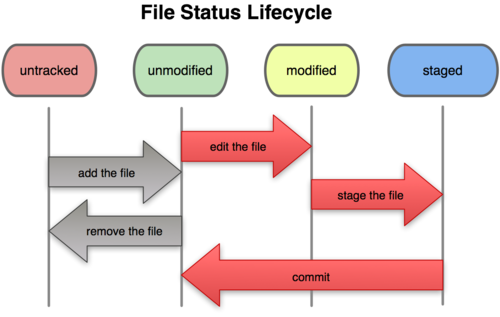
\includegraphics[width=\textwidth]{img/file_lifecycle}
        \caption[format=empty]{Quelle: \url{http://progit.org}}
      \end{figure}
    \end{column}
    \begin{column}{0.65\textwidth}
      \begin{itemize}
        \item nicht versioniert (\textbf{untracked})
        \item versioniert, aber unverändert (\textbf{unmodified})
        \item versioniert und verändert (\textbf{modified})
        \item versioniert, verändert und in der „staging area“ (\textbf{staged})
      \end{itemize}
    \end{column}
  \end{columns}
\end{frame}

\begin{frame}[fragile]{typischer Workflow}
  \begin{itemize}
    \item Initialisieren eines git Repositories
    \begin{lstlisting}
cd meinprojekt
git init
    \end{lstlisting}
    \item Dateien der „staging area“ hinzufügen
    \begin{lstlisting}
git add <file>
    \end{lstlisting}
    \item Änderungen in der „staging area“ committen
    \begin{lstlisting}
git commit -m 'initial commit'
    \end{lstlisting}
    \end{itemize}
\end{frame}

\begin{frame}[fragile]{Änderungen betrachten}
  \begin{itemize}
    \item Den aktuellen Status des Repositories betrachten
    \begin{lstlisting}
git status
    \end{lstlisting}
    \item Änderungen im Arbeitsverzeichnis betrachten
    \begin{lstlisting}
git diff
    \end{lstlisting}
    \item Änderungen betrachten, die sich bereits in der „staging area“ befinden
    \begin{lstlisting}
git diff --cached
    \end{lstlisting}
  \end{itemize}
\end{frame}

% vim: tabstop=2 expandtab shiftwidth=2 softtabstop=2 autoindent
